前文已经介绍了系统总体设计(包含硬件设计及软件设计)和相关算法。本
小节将结合前文,具体实现一个停车管理系统。本系统以树莓派3b+为硬件平台利用python为编译环境实现。另外也设计了两个云端服务器:其中一个是车牌识别云端服务器,用来将树莓派摄像头拍下的照片进行处理得出车牌号码;另外一个是停车管理系统云端服务器,用来管理车辆。实现流程图如图\ref{fig:进出库总体任务分析流程图}所示。

\begin{figure}[htbp]
	\centering
	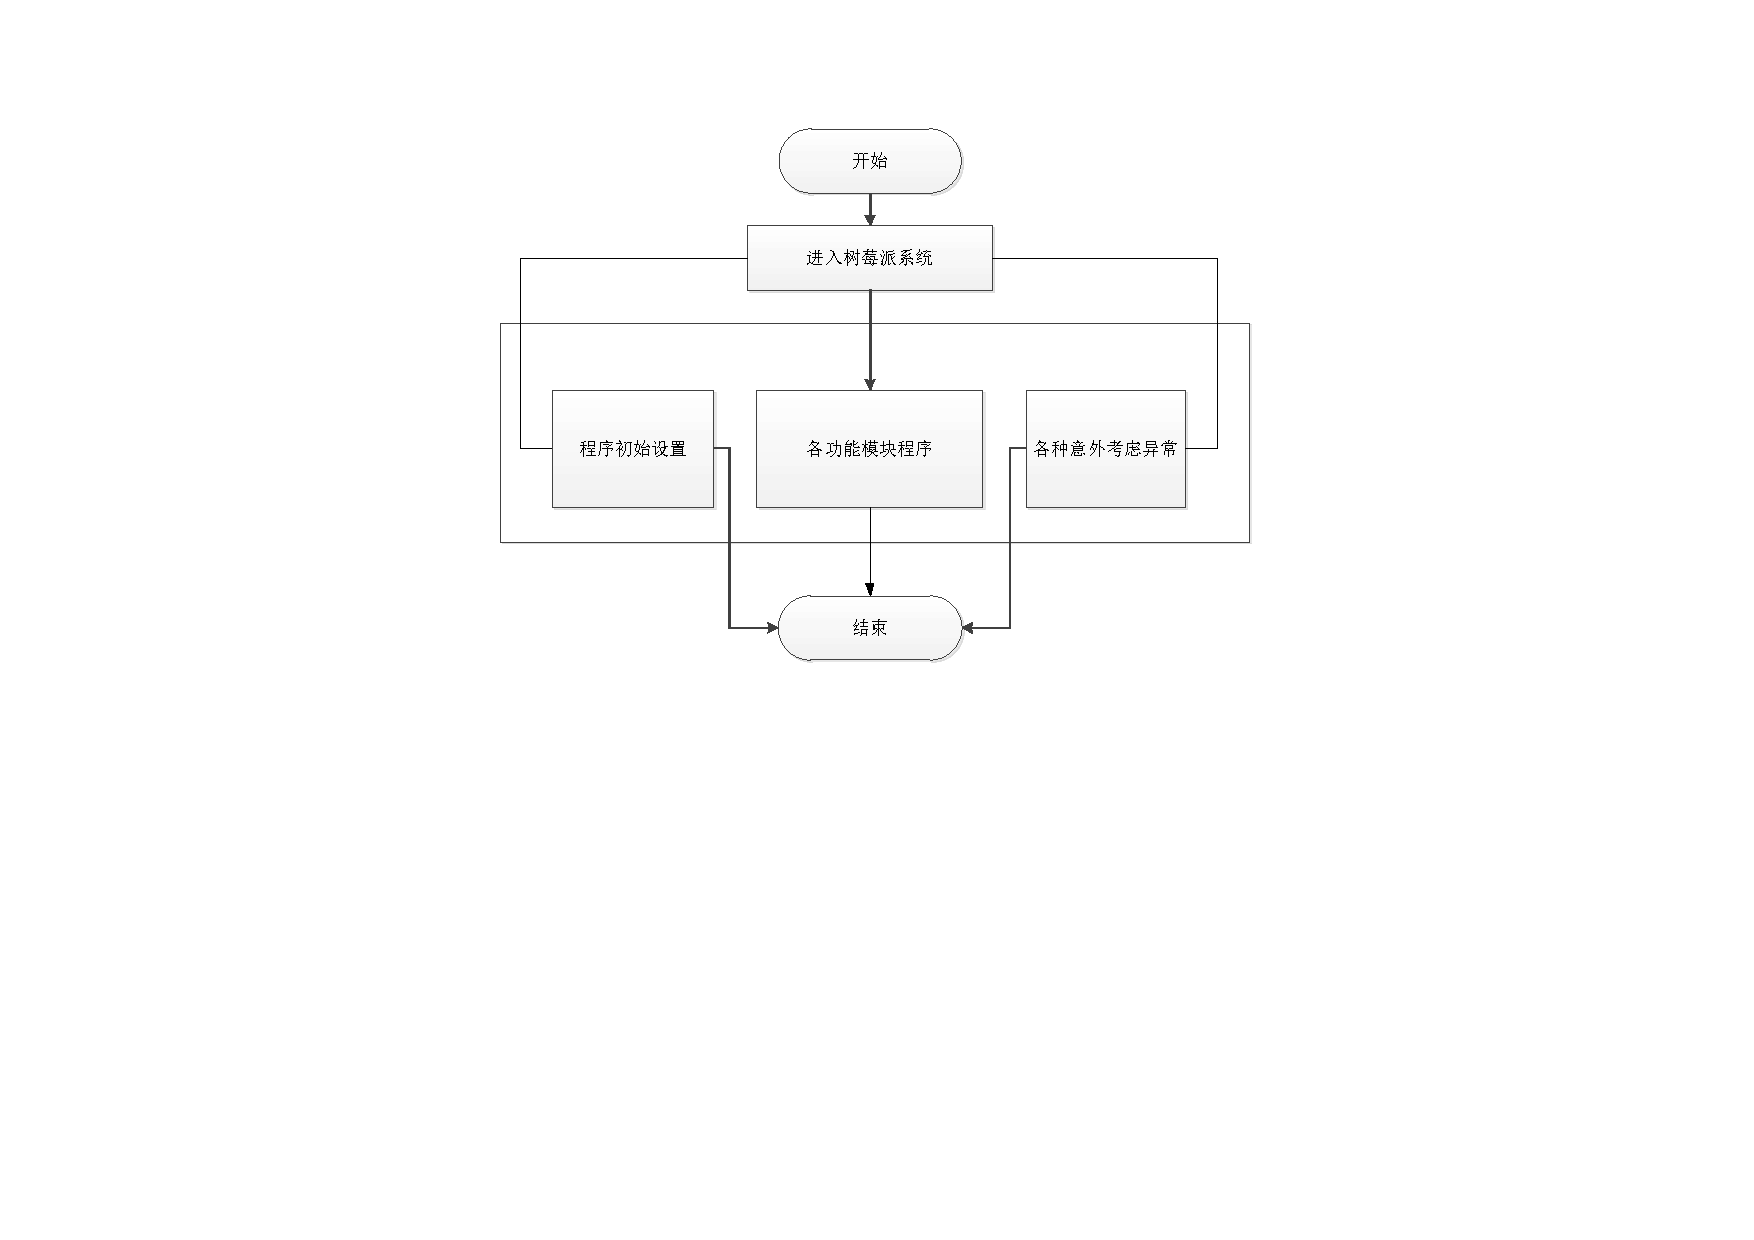
\includegraphics[width=\textwidth]{figure/software-7.pdf}
	\caption{进出库总体任务分析流程图}\label{fig:进出库总体任务分析流程图}
\end{figure}

\subsubsection{程序初始值设置(附录\ref{apdx:__init__.py}、附录\ref{apdx:config.py})}
程序首先定义了电机的管脚N1、N2、N3与N4分别为GPIO(29)、GPIO(31)、GPIO(33)和GPIO(35)。杆前红外线的避障管脚AvoidSensorfor定义为GPIO(40),杆后红外线的避障管脚AvoidSensorbac定义为GPIO(38)。程序还定义了电机四个管脚与两个红外管脚的GPIO口初始化程序。

\subsubsection{电机不同运转状态设置(附录\ref{apdx:motor.py})}
在motor.py中,定义了电机的不同运转状态程序,第一个函数SetStep()是定义电机四个管脚的输出电平,电机顺时针旋转、逆时针转动以及停止都需要调用该函数。后三个函数调用SetStep()时,SetStep()的设置得需要遵循如表4-1的步进电机驱动原理表,每次将四个GPIO端口按表4-1的步进电机驱动原理表依次设置好电平后,可以通过设置sleep()函数的时间来控制转速与方向,这样后三个函数便可以通过设置SetStep()分别实现顺时针旋转、逆时针旋转与停止。

\subsubsection{相机拍照传送(附录\ref{apdx:camera.py})}
相机拍照部分写成三个函数:capture、detect、capture\_detect。主程序里主要运行capture\_detect(),该函数里包括capture(path)与返回detect(path)。该函数运行时,调用capture(path)捕捉到照片存放到本地当前目录,文件设为image.jpg,然后返回capture(path),capture(path)将当前目录的照片发送至车牌识别云端,若从云端返回的车牌号为空,则返回0;若不为空,则返回该车牌号码。

\subsubsection{树莓派与服务器的通信(附录\ref{apdx:CarEnter.py}、附录\ref{apdx:CarOut.py})}
\begin{enumerate}
    \item 树莓派与车牌识别云端的通信:将树莓派拍下的图片作为写入字典中,然后传给传给requests.post()的参数,最后用json.loads()解码json数据;
    \item 树莓派与停车管理系统云端的通信requests.get()用于请求目标网站,类型是一个HTTPresponse类型,这里的request获取的是剩余车位的值。
\end{enumerate}

\subsubsection{车入库具体流程代码分析(附录\ref{apdx:CarEnter.py}、附录\ref{apdx:CarOut.py})}
检测车进:红外模块的避障引脚一旦出现低电平,则需要摄像头开启抓捕拍照,而且仅仅拍一张照片,将其存放到树莓派本地。紧接着照片被送往云端识别,会立即返回车的车牌号码。可能会出现未识别的情况,只要车不退回,系统会一直拍照直至能够产生车牌号码,除非用户自己离开系统放弃拍照。若产生正确的照片会被发往停车管理系统云端,返回剩余车位不为0时则杆立即抬起,车开始开进车库,第二个红外模块检测到车身时直至检测不到杆落下。

检测车出:出库程序运行时,当红外模块检测到车身时,则摄像头开启抓捕拍照。类似于车进库的操作,照片被送往云端识别,云端会返回车的号码。若是没有识别会会一直识别,若是长久不能识别,车主此时必须打电话给管理员。若是车牌识别成功,会立即发往停车管理系统云端,云端返回一个SVG字符串格式的二维码。

在本地将此格式转换为图片格式即为付款二维码。车主需要付款扫二维码并付款成功后杆才可抬起,离开的时候第二个红外模块第一次检测到车身不落杆,直到
避障管脚输出True时,杆才开始落下,此时车已经安全离开。
